\section{BSPro - A Third Bachelor Semester Project in BiCS-land}
\subsection{Requirements ($\pm$ 15\% total words)}

In this section we describe the algorithms which we implement in our chat application. Later on, we carry on a speed comparison between them. 

Ciphers have been used long before apparition of computers. During Roman times, Julius Caesar invented an encryption for his private correspondence. Today, it is known as the Caesar cipher. Given the English alphabet, the cipher shifts a letter from the alphabet three places to the right, i.e. A is encrypted as D, B as E, etc. It is a monoalphabetic cipher. To decrypt the message, the other party needs to know both the algorithm and the shifting number. The secret key shared by the sender and the recipient of the message is k=3. Breaking the Caesar Cipher can be done by testing all possible shifts. Since an alphabet of length 26 is used, we have to test 26 shifts. 

ROT13 is a simple monoalphabetic substitution cipher, a special class of Caesar cipher, that encodes a certain letter with another letter that is 13 positions after it. Only those letters which occur in the English alphabet are affected. Numbers, symbols, whitespace, and all other characters are left unchanged. It is an example of a cipher providing weak encryption, since both operations encryption and decryption are identical. Hence, this cipher is its own inverse. Because there are 26 letters in the English alphabet, if we wish to apply twice 13 it would give us one shift of 26. Thus, it leads us back to the original text. Moreover, the direction of the shift is of no importance, since it will always give the same output \cite{swenson2008modern}.
ROT13 is used in online forums as a means of hiding spoilers, punchlines, puzzle solutions, and offensive materials from the casual glance. Furthermore, it has inspired a variety of letter and word games online \cite{wikirot13}. 

Another cipher our project deals with is the block cipher Data Encryption Standard (DES). In DES, we put a 64 bit block of plaintext. Its key, doing the processing, is 64 bit which is 8 bytes. For each byte there is one parity bit, therefore, the value in the key is only 56 bits. Thus, there are 2 to the power of 56 different keys. The output ciphertext is a 64-bit block. 
Figure \ref{fig:desround} shows a DES Round Encryption. From the 56-bit key, 16 bits are generated (one for each round). See Figure \ref{fig:destopview} for a DES Top View. Each DES round works consecutively, has the same operations and uses a different key. Each round uses a combination of proper substitution, where we take some bits, substituted with another combination of bits. Each DES round takes as an input the ciphertext produced by the previous round and outputs the ciphertext for the next round. The input is divided into a left half and a right half. The output left half is just the right half of the input. The right output is the result of XOR-ing the left half of the input and the output of the Mangler Function. This function takes as an input the 32-bit right half, expands it to 48-bit (bit-wise operation), then XORs it to 48-bit key, and finally uses the S-Boxes to substitute the 48-bit value into a 32-bit value. 
The algorithm process of decryption in DES is the same as the encryption process. It uses the ciphertext as an input to DES but the keys are run in reversed order, i.e. k = 16 is used as the first round of decryption, k = 15 is used as a second round of decryption and so on, so forth. 
Diffusion is one of the principles in encryption. It is achieved through permutation (initial transposition). Permutation works by changing the position of the bits in DES. The mixed bits are taken to a sub-box which receives the 56-bit key and the 64-bit plaintext. Once it completes processing, it outputs the 64 bits into another transposition subsection, which in turn produces a 64-bit ciphertext. 
The larger the block size, the key size and number of rounds means greater security. The two most significant attacks applicable to symmetric-key block ciphers are differential cryptanalysis and linear cryptanalysis. The former is a chosen plaintext attack, in which the attacker is able to select inputs and examine outputs in order to derive the key. The latter is a known plaintext attack: that is, it is premised on the attacker having information on a set of plaintexts and the corresponding ciphertexts. However, according to Stallings, DES has proven to be resistant to them \cite{stallings2011-a}. By 1999, a computer could try every possible key in a couple of days rendering the cipher insecure.

AES supports a block length of 128 bits and key lengths of 128, 192, and 256 bits. Figure \ref{fig:aes} shows a simplified concept behind AES algorithm. Thus, brute-force attacks are much harder to be launched against it. AES chops data up into 16-byte blocks, transferred to a \emph{state array}, and then applies a series of substitutions (e.g. \emph{substitute bytes}, \emph{MixColumns}) and permutations (e.g. \emph{ShiftRows}), based on the key value. We note that the state array undergoes various modifications throughout both encryption and decryption. Moreover, that way, it obscures the message, by adding diffusion, confusion and non-linearity and repeating the processes ten (for a 16-byte key) or more times (12 rounds for 24-byte key; 14 rounds for a 32-byte key) for each block. In order to \emph{substitute bytes}, an S-box is used to perform a byte-by-byte substitution of the block. The other substitution, called \emph{MixColumns}, utilizes arithmetic over ($2^{8}$) \cite{stallings2017-a}. In fact, all encryption algorithms necessitate arithmetic operations. The key is expanded into an array of key schedule four-byte words. Employing a bitwise XOR of the current block with part of the expanded key is a stage called \emph{AddRoundKey}, solely used on the key. Therefore, the cipher is locked around this stage adding to the security of the AES encryption.  At the end, the state of the plaintext is copied to an output matrix where the bytes are ordered in a column. Similarly, the bytes of the expanded key, which form a word, are placed in the column of the matrix. Today, AES is used everywhere, from encrypting files and sensitive data, transmitting data over WiFi with WPA2, to accessing websites using HTTPS. 

\subsection{Design ($\pm$ 20\% total words)}

The technical part of our project consists of creating a chat application. Our source code editor is Visual Studio Code and we program in Python. We create a TCP server as well as a TCP client that connects to the server. 
To implement the client, we use a socket module, imported from Python's standard library. It serves as a communication endpoint with two parameters:
\begin{verbatim}
s= socket.socket
    (socket.AF_INET, socket.SOCK_STREAM)
\end{verbatim}
The first parameter \textit{AF\_INET} stands for IPv4, i.e., the connection type we want to use, and the second parameter, \textit{SOCK\_STREAM}, means we are going to use TCP connection. We specify a variable for port number (on which the server is running) and IP, which holds the IP of the host machine it is running on. We use \textit{gethostbyname} to look for the host’s IP since the host machine, used to conduct the technical simulation, does not have a fixed IP address and often when it reconnects to an Internet connection is assigned a new IP address.
\begin{verbatim}
ip = str(socket.gethostbyname
           (socket.gethostname()))
port = 1234
\end{verbatim}
Once the port and IP address are known, we can connect to the server by passing the function to a data structure:
\begin{verbatim}
s.connect(((ip, port))
\end{verbatim}

To implement the server, we use a socket module that serves as a communication endpoint with two parameters:
\begin{verbatim}
s= socket.socket
    (socket.AF_INET, socket.SOCK_STREAM)
\end{verbatim}
For the client to be able to connect to the server, it should make use of the same port number. When the port and host have been bounded, we can listen to incoming connections with socket variable s and calling listen on it:
\begin{verbatim}
s.listen(10)
\end{verbatim}
We pass the variable 10 which means that up to 10 different connections can be queued for the server to handle the requests. To accept requests from outside, we use connection variable and address variable:
\begin{verbatim}
conn, addr = s.accept()
\end{verbatim} 
which stores the IP import of the client, trying to connect and we call accept on the socket we have created. Upon establishing connection, the client can send information to the server that will cause it to echo back the data. The server can receive data up to size 4096 from the client:
\begin{verbatim}
incoming_message = conn.recv(4096)
\end{verbatim} 
Afterwards we can close the connection between client and server
\begin{verbatim} 
conn.close()
\end{verbatim} 
on the server side, as well as close the socket itself as it allows connections to exist, on the client side,
\begin{verbatim} 
s.close()
\end{verbatim}
\par
For our project, we aim at implementing several encryption and decryption applications in Python. The client stores the encryption algorithms, whereas the server holds the decryption methods. We make use of Caeser cipher, ROT13, DES, and AES.
DES and AES have been implemented through the means of the crypto library “PyCryptodome”\cite{pycryptodome}. It is a self-contained Python package of low-level cryptographic primitives \cite{pycryptodome}. It supports PyPy, Python2 and Python3. PyCryptodome can be used as a replacement for the old PyCrypto library. We install all modules under Crypto package with pip3 install pycryptodome.  However, having both PyCrypto and PyCryptodome installed at the same time is not a good idea as they will interfere with each other. If, however, one insists on having them both, it would be best to deploy them in a virtual environment. To have an independent library of the old PyCrypto, it suffices to type the following command in Terminal shell:
\begin{verbatim}
pip3 install pycryptodomex
\end{verbatim} 
and all modules are installed under Cryptodome package. PyCrypto and PyCryptodome can still coexist.


\subsection{Production ($\pm$ 20\% total words)}

We implement all encryption algorithms with Python programming language. Table \ref{algorithms} shows the settings of the algorithms we are implementing.

\begin{table}[h!]
\begin{tabular}{|c|c|c|}
\hline
\textbf{Algorithm} & \textbf{Key size} & \textbf{Type of cipher}  \\ \hline
Caesar cipher      & 3                 & Letter substitution      \\ \hline
ROT13              & 13                & Letter substitution      \\ \hline
DES                & 64 bits           & Block cipher of size 64  \\ \hline
AES                & 256 bits          & Block cipher of size 256 \\ \hline
\end{tabular}
\caption{Algorithm settings}
\label{algorithms}
\end{table}

Caeser cipher is a substitution cipher and a type of shift cipher. Shift ciphers work by using the modulo operator to encrypt and decrypt messages. In the following lines we demonstrate the algorithm. We take an alphabetic message (a to z). We set the key, an integer from 0 to 25, since there are 26 letters in English alphabet, to be equal to 3.To encrypt, we do a right-shift letter by letter by the value of key mod 26. To decrypt, a left-shift of the message letter by letter is performed, subtracting the value of key and taking the modulus 26. The characters are calculated in the input string as this will be used for the number of iterations that need to be done to encrypt and decrypt everything (one character at a time). Our code can be presented as follows: for every letter in the message, we find the letter that matches its position in the alphabet starting from 0. We calculate
\begin{verbatim}
newPosition = (position + key) mod 26
\end{verbatim} 
then convert \textit{newPosition} into a letter that matches its order in the alphabet starting from 0. During the iteration it uses the alphabets' string as its base for shifting the characters, skipping those not part of the base string (such as numbers and symbols) to keep the structure of the input intact.
Finally it outputs the ciphertext (\textit{newMessage}) for us to use. The decryption process is similar; however, instead of adding the key, we subtract it during the modular operation.

ROT13 is a special case of Caeser cipher, therefore, both codes are similar. However, ROT13 is implemented by setting the value of the key to 13. The key is used by both encryption and decryption algorithms to shift the plaintext by 13 characters. Firstly, we initialize the letters. An ASCII table contains upper letters \textit{A-Z} from positions 65 to 90, whereas, lower case letters \textit{a-z} are within the range of 97 to 122. The \textit{chr()} function is the opposite of \textit{ord()}. The \textit{ord()} function returns an integer representing the unicode code point of a character string. For example, \textit{ord('z')} returns the integer 122. On the other hand, \textit{chr()} returns the string character whose Unicode code point is an integer. For instance, \textit{chr(122)} returns string ‘z’. What makes this technique fairly simple is that if we implement rot13() on the ciphertext, then we get back the plaintext since each letter in the text is rotated by the same shift. Thus, the same \textit{encrypt\_rot13()} function is defined for both encryption and decryption operations to rotate the letters. Depending on the provided letter (lower or upper case), the rot13 function encrypts according to the ASCII table and returns the ciphertext. 

To implement DES, we import DES functional dependency from Cryptodome library module. Then we create and specify a fixed \textit{key = “mysecret”} of length 8 bytes, a password that shall be used to encrypt the text. We have created a pad function, \textit{despad}, taking as input \textit{plaintext}. Within this function, we run a while loop checking the length of text mod 8, i.e. the modulus divides it and shows the remainder. If remainder is not equal to zero, we add a blank space at the end of text such that it becomes multiple of 8 (e.g., 8, 16, 24, 32, etc.). Otherwise the encryption is not going to work as DES encryption algorithm, takes input in 8 bytes. For instance, if we type ‘abcd’, the function adds four empty spaces at the end of ‘abcd’ to make sure it is a total of 8 characters/bytes. Then, we create an object, called \textit{des}. We use function \textit{new()} of module DES that takes two parameters: key and \textit{DES.MODE\_ECB} which is the encryption mode. We have created a variable taking an input from the client that shall be encrypted. The variable  \textit{padded\_text} uses the despad() function on the client's input to make sure it is a multiple of 8 and if necessary adds empty spaces to conform to the multiple condition. Next, we have created the variable \textit{encrypted\_text} that uses the function \textit{encrypt()} on the \textit{padded\_text} and turns it into an encrypted cipher. To represent ciphertexts, it is more readable to use hex strings rather than bytes. Moreover, hex() makes it easier to parse the decryption input, implemented in the server. To be sure that data remains intact without modification during transfer from client to server, we need to encode it. To reverse the process, the server needs to decode the message. In order to decrypt, we run \textit{des} submodule from the library and pass function  \textit{decrypt()} on it. Since we have used padding before encryption, we need to unpad the recovered cleartext by using rstrip(). 

AES has been implemented using the \textit{PyCryptodome} library. We import the module AES along with the hash package and hash object \textit{SHA-256}. In function \textit{make\_key()}, SHA-256 produces a 256-bit digest of a password. \textit{Digest()} returns a binary digest of the message that has been hashed. Since \textit{digest()} produces a random output it is impossible to derive the original input data. On the client side, the \textit{aesencrypt()} function has a pad variable which appends to the back as many bytes we need to reach the next 16-byte boundary, before encrypting the bytes message. On the server side, an unpad function is used to reverse the padding executed by the client. The \textit{block\_size} is the size of the message block in bytes. The IV (initialization vector) is a unique and random piece of data used to initialize the processing. This setting does not allow an attacker to get relations between encrypted messages segments. The IV does not need to be private so that we can send it with the ciphertext without risk. Its length is equal to 16 bytes. The key and IV have been loaded on separate files and are used for both encryption and decryption. The IV is written and overwritten in a file each time it is used to encrypt a message. And it is being read from the file during decryption by the server. When we couple the key with the mode of operation CBC (Ciphertext Block Chaining), where the IV is randomly generated for each new message. Thus, we can encrypt a lot of data under the same key. CBC requires the length of plaintext and ciphertext to be always a multiple of 16 bytes. The function \textit{new()} instantiates a new object for the AES algorithm. It has 3 parameters: key (in bytes), mode \textit{(MODE\_CBC)} and IV (in bytes as a read-only attribute). The function \textit{new()} returns a CBC cipher object. To encode and decode the message, base64 has been used. It allows to transfer over a medium relying on textual data by converting from binary data to text strings and vice versa. The method \textit{encrypt()} (and likewise \textit{decrypt()}) of a CBC cipher object expects data to have length multiple of the block size, i.e., 16 bytes for AES. The message is being translated from a Unicode string into a sequence of bytes through UTF-8 (Unicode Transformation Format) encoding. \textit{Encode(“utf-8”)} and \textit{Decode(“utf-8”)} return byte representations of the unicode string, encoded in UTF-8.

\subsection{Assessment ($\pm$ 15\% total words)}

We have used a TCP transport-layer protocol with the same IP address and port number for both client and server. We have shown a secure communication over the Internet between a client and a server, having the choice to encrypt and decrypt with four different algorithms. We highlight that both client and server should support the same set of encryption algorithms, modes of operation, as well as keys, set for encryption and decryption processes. In this section, we assess the encryption and decryption operations utilized by the algorithms. We also take into account the modes of operations and supplementary features such as IV and key generation. Furthermore, we conduct a performance analysis choosing as a factor the speed necessary to encipher and decipher information. 

In general, the mode of operation plays an important role in the security of the cipher. We have used two block ciphers, DES and AES. ECB (Electronic Code Book), used along DES in our project, splits up the plaintext into blocks and encrypts them independently of each other in a parallel operation. This is an advantage of ECB. ECB does not use an initialization vector to launch the encryption. Thus, it executes the same algorithm to encrypt data. However, when multiple messages are encrypted, ECB cannot be considered secure, because identical plaintext blocks result in identical ciphertext, also known as deterministic encryption. Hence, repetition makes it easier for an attacker to guess the original message. CBC cannot operate in parallel since it waits on finishing encryption on each block. CBC, used along AES in our project, introduces an initialization vector (IV), which alters the plaintext before the start of the encryption process. The vector ensures that the initial ciphertext blocks are different even with an identical plaintext. To accomplish this, the IV is unpredictable, unique and cryptographically random for each separate key to avoid deterministic encryption. As both the encryption and decryption need to be performed using the same unique IV.  If we use a different IV in decryption, we would get a garbled message indicating an erroneous use of IV. Furthermore, the IV must be of the same length as the block size (e.g., given 64-bit block size, 64-bit IV, etc.) As mentioned earlier, when a predictable IV is used, CBC is considered vulnerable as plaintexts could be deduced. Hence, the IV cannot be transmitted alongside the cipher. The IV is the result of the previous encrypted block, XORed with the plaintext block before encryption. Hence, with CBC, every block depends on the output of the previous block. Nevertheless, the disadvantage of this property is that if there is an error or failure in a given block, it will result in the following block as well. The key in AES is hashed to provide a 256-bit output, then the hash is encrypted, and a 256-bits encrypted output is produced. The IV is then used to encrypt the next 256-bits. This results in a chaining algorithm.
Considering the comparison between the two modes of operation, it is not a good idea to use ECB for message confidentiality as it is a rather simple and raw mode for a block cipher. Instead, we can turn to CBC and its random use of IV. 

We conducted a performance analysis of the implemented algorithms. The simulation was administered on a 3,1 GHz Intel Core i7 processor with 16 GB 1867 MHz DDR3 memory. The experiments have been performed couple of times to assure that the results are consistent and are valid to compare the different algorithms. The time needed for each method to encrypt and decrypt a message of 100 bytes was measured in seconds. The message is the following: \textit{This is a 100-byte message, measuring the time it takes to encrypt and decrypt it by each algorithm}. It is imperative to note that we prepared the sentence in advance and copied-pasted it to the console. If we take the time to write a message on the spot, the time measurements will differ. 

\begin{figure}[h!]
  \centering
  \begin{subfigure}[b]{1.0\linewidth}
    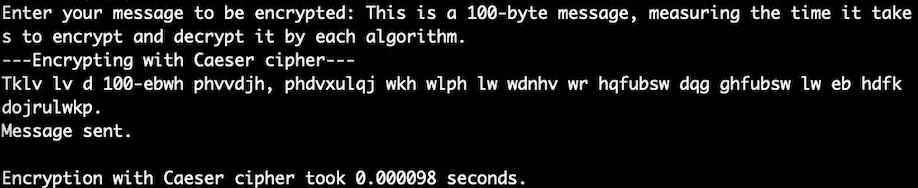
\includegraphics[width=\linewidth]{caesarencrypt.jpg}
    \caption{Caesar encryption time.}
  \end{subfigure}
  \begin{subfigure}[b]{1.0\linewidth}
    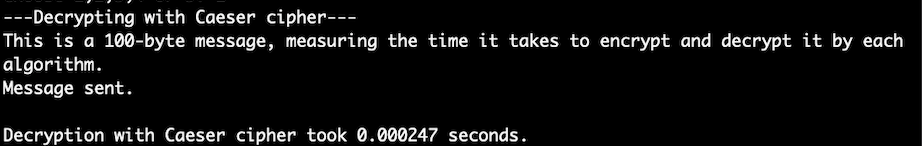
\includegraphics[width=\linewidth]{caesardecrypt.jpg}
    \caption{Caesar decryption time.}
  \end{subfigure}
  \caption{Caesar cipher Encryption/Decryption time of a 100-byte message.}
  \label{fig:caesar}
\end{figure}

\begin{figure}[h!]
  \centering
  \begin{subfigure}[b]{1.0\linewidth}
    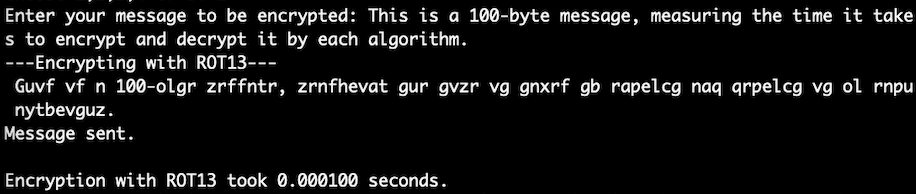
\includegraphics[width=\linewidth]{rot13encrypt.jpg}
    \caption{ROT13 encryption time.}
  \end{subfigure}
  \begin{subfigure}[b]{1.0\linewidth}
    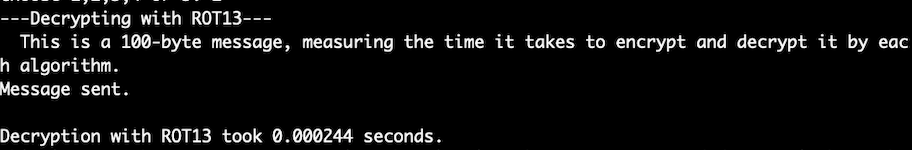
\includegraphics[width=\linewidth]{rot13decrypt.jpg}
    \caption{ROT13 decryption time.}
  \end{subfigure}
  \caption{ROT13 Encryption/Decryption time of a 100-byte message.}
  \label{fig:rot13}
\end{figure}

\begin{figure}[h!]
  \centering
  \begin{subfigure}[b]{1.0\linewidth}
    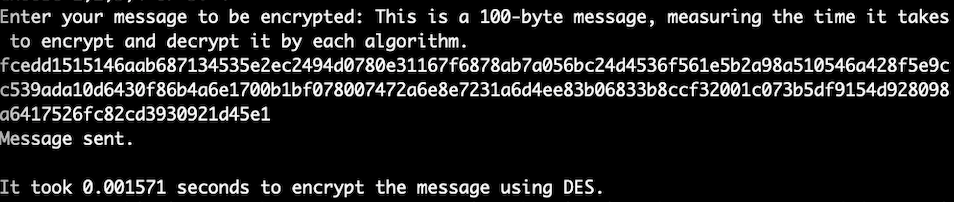
\includegraphics[width=\linewidth]{desencrypt.jpg}
    \caption{DES encryption time.}
  \end{subfigure}
  \begin{subfigure}[b]{1.0\linewidth}
    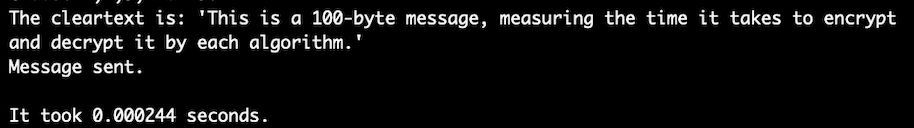
\includegraphics[width=\linewidth]{desdecrypt.jpg}
    \caption{DES decryption time.}
  \end{subfigure}
  \caption{DES Encryption/Decryption time of a 100-byte message.}
  \label{fig:des}
\end{figure}

\begin{figure}[h!]
  \centering
  \begin{subfigure}[b]{1.0\linewidth}
    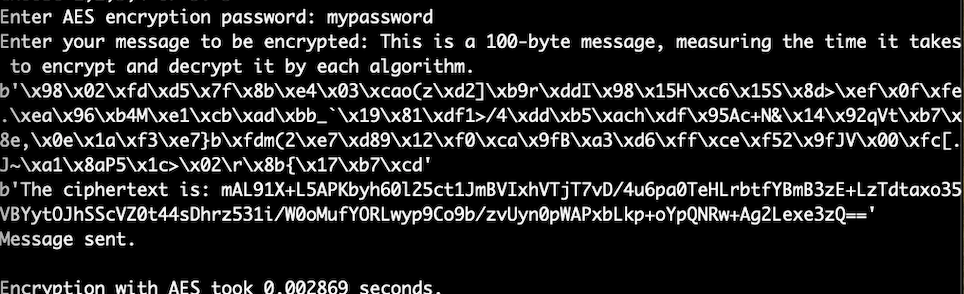
\includegraphics[width=\linewidth]{aesencrypt.jpg}
    \caption{DES encryption time.}
  \end{subfigure}
  \begin{subfigure}[b]{1.0\linewidth}
    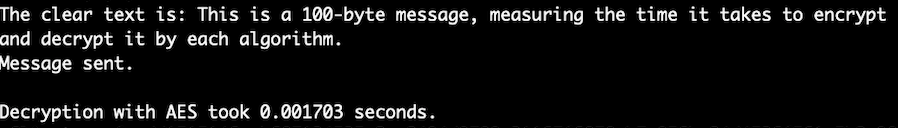
\includegraphics[width=\linewidth]{aesdecrypt.jpg}
    \caption{DES decryption time.}
  \end{subfigure}
  \caption{AES Encryption/Decryption time of a 100-byte message.}
  \label{fig:aes}
\end{figure}



\begin{table}[h!]
\begin{tabular}{|l|c|c|}
\hline
\multicolumn{1}{|c|}{} & Time for encryption & \multicolumn{1}{l|}{Time for decryption} \\ \hline
Caesar cipher & 0.000098 & 0.000247 \\ \hline
ROT13 & 0.000100 & 0.000244 \\ \hline
DES & 0.001571 & 0.000244 \\ \hline
AES & 0.002869 & 0.001703 \\ \hline
\end{tabular}
\caption{Comparative execution time (in seconds) of implemented algorithms}
\label{results}
\end{table}



Figures 1 to 4 represent the time it took for each algorithm to encrypt and decrypt the 100-byte message. Table \ref{results} summarizes the results of the experiment. The security features of each algorithm as their strength against cryptographic attacks is already known and discussed. The factor we have chosen to determine the performance is the speed to encrypt and decrypt the data of size 100 bytes. It is easy to observe that Caesar cipher and ROT13 performed similarly in time, as expected, since they are identical cases. Moreover, DES outputs faster than AES because it is not relying on initialization vector (iv) and because the ECB mode is simpler than CBC, but these make it a weak encryption mechanism. AES performed poorly in terms of speed since CBC mode adds extra processing time due to its key-chaining nature. Nevertheless, CBC mode of operation is better than ECB and for that AES is considered the most secure of all four algorithms. We note that AES needs almost twice the time of DES to encrypt the 100-byte message and roughly ten times to produce the plaintext. In addition, AES consumes more resources and requires more processing time since it utilizes an iv and CBC mode. Overall, the slow performance of AES can be considered as negligible for applications that require secure transmission of sensitive data over the Internet.

In addition, to prevent access to the message from the outside while transferring information between clients and server, we should not store any data as plaintext. The reason being is that any stored piece of information can be accessed during an attack on the server, such as a social engineering or man in the middle attack. Another remark to be made is to never create our own cryptography security schemes and to never implement an existing standard on our own. We will most probably do major security mistakes leading to insecure applications. However, for the purpose of academic education, we could not obey this rule of law. 
As a future work, we could simulate a couple of attack scenarios such as a frequency letter analysis (on Caesar cipher and ROT13), man-in-the-middle attack or brute force (on both AES and DES) and test their success. 


\section*{Acknowledgment}
The authors would like to thank the BiCS management and education team for the amazing work done.